\documentclass[tikz]{standalone}
\usepackage[utf8]{inputenc}

\begin{document}
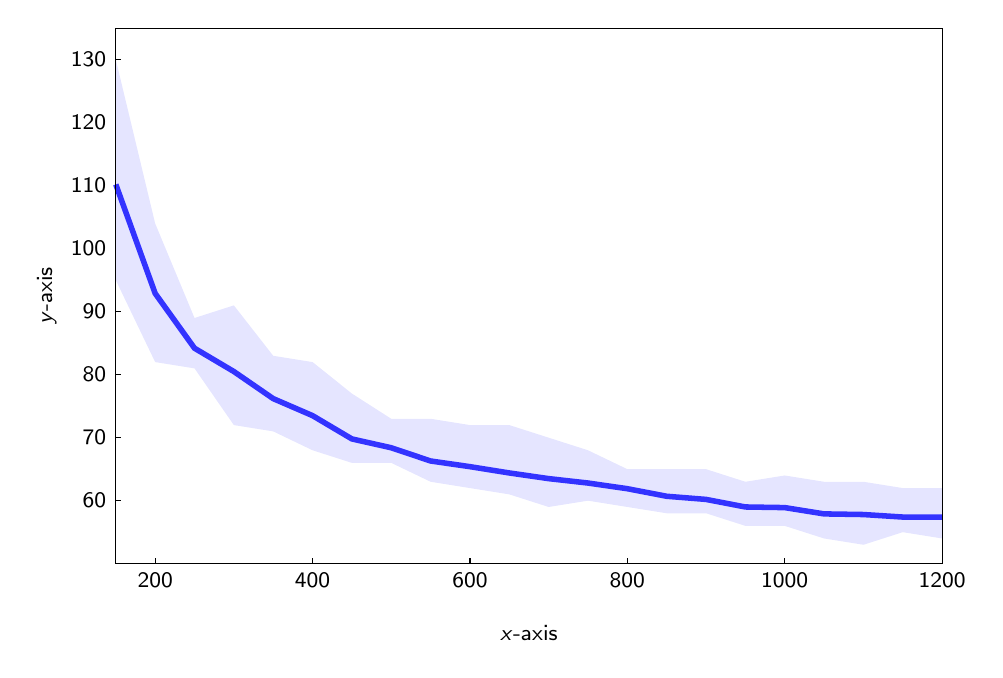
\begin{tikzpicture}[x=.01cm,y=0.08cm]
\foreach \x in {200, 400, ..., 1200} {
\draw (\x, 50) --++ (0,2pt);
\node[below] at (\x, 50) {\footnotesize\sffamily \x};
}

\foreach \y in {60, 70, ..., 130} {
\draw (150, \y) --++ (2pt,0);
\node[left] at (150, \y) {\footnotesize\sffamily \y};
}

\fill[color=blue!10] plot coordinates {(150, 95) (200, 82) (250, 81) (300, 72) (350, 71) (400, 68) (450, 66) (500, 66) (550, 63) (600, 62) (650, 61) (700, 59) (750, 60) (800, 59) (850, 58) (900, 58) (950, 56) (1000, 56) (1050, 54) (1100, 53) (1150, 55) (1200, 54) (1200, 62) (1150, 62) (1100, 63) (1050, 63) (1000, 64) (950, 63) (900, 65) (850, 65) (800, 65) (750, 68) (700, 70) (650, 72) (600, 72) (550, 73) (500, 73) (450, 77) (400, 82) (350, 83) (300, 91) (250, 89) (200, 104) (150, 130)};

\draw[line width=2pt, color=blue!80] plot coordinates {(150, 110.2) (200, 92.9) (250, 84.2) (300, 80.5) (350, 76.2) (400, 73.5) (450, 69.8) (500, 68.4) (550, 66.3) (600, 65.4) (650, 64.4) (700, 63.5) (750, 62.8) (800, 61.9) (850, 60.7) (900, 60.2) (950, 59.0) (1000, 58.9) (1050, 57.9) (1100, 57.8) (1150, 57.4) (1200, 57.4)};

\draw (150,50) -- node[pos=0.5, yshift=-25pt] {\footnotesize\sffamily \textit{x}-axis} (1200,50) -- (1200, 135) -- (150, 135);
\draw (150,50) -- node[pos=0.5, xshift=-25pt, rotate=90] {\footnotesize\sffamily \textit{y}-axis} (150,135);
\end{tikzpicture}
\end{document}